%%==================================================
%% chapter02.tex for SJTU Master Thesis
%% Encoding: UTF-8
%%==================================================

\chapter{Trivium算法}
\label{chap:Trivium}

\begin{algorithm}
	\caption{Trivium算法最小阶数计算}
	\label{algo:trivium_maple}
	\begin{algorithmic}
		
		\FOR {$w1 \leftarrow 1$ \TO $6$}
			\FOR {$w2 \leftarrow (w1 + 1)$ \TO $7$}
				\FOR {$w3 \leftarrow (w2 + 1)$ \TO $8$}
					\FOR {$w4 \leftarrow (w3 + 1)$ \TO $9$}
						\FOR {$w5 \leftarrow (w4 + 1)$ \TO $10$}
							\FOR {$w6 \leftarrow (w5 + 1)$ \TO $11$}
								\FOR {$w7 \leftarrow (w6 + 1)$ \TO $12$}
									\FOR {$w8 \leftarrow (w7 + 1)$ \TO $13$}
										\FOR {$w9 \leftarrow (w8 + 1)$ \TO $14$}			
											\STATE {$(w_{1}, w_{2}, \ldots, w_{9}) \leftarrow (w1, w2, \ldots, w9)$}
											\STATE $A \leftarrow Matrix(w_{9}*3)$
											\STATE $A[1][w_{9}*3] \leftarrow 1$
											\FOR {$i \leftarrow 2$ \TO $(w_{9} * 3)$}
												\STATE $A[i][i - 1] \leftarrow 1$
											\ENDFOR	
											\STATE $A[3*w_{3}+1][3*w_{1}] \leftarrow 1$
											\STATE $A[3*w_{3}+1][3*w_{5}] \leftarrow 1$
											\STATE $A[3*w_{6}+1][3*w_{4}] \leftarrow 1$
											\STATE $A[3*w_{6}+1][3*w_{8}] \leftarrow 1$
											\STATE $A[1][3*w_{2}] \leftarrow 1$
											\STATE $A[1][3*w_{7}] \leftarrow 1$
											\STATE $f \leftarrow charpoly(A, x) mod \quad 2$
											\IF {$Divide(f,(x^{3}+1)^{3},'g') mod \quad 2$}
												\STATE $g \leftarrow algsubs(x^{3}=x, g)$
												\IF {$Primitive(g) mod \quad 2$}
													\STATE $output(w)$
												\ENDIF
											\ENDIF
										\ENDFOR
									\ENDFOR
								\ENDFOR
							\ENDFOR
						\ENDFOR
					\ENDFOR
				\ENDFOR
			\ENDFOR
		\ENDFOR
		
	\end{algorithmic}
\end{algorithm}

\begin{figure}[!htp]
	\centering
	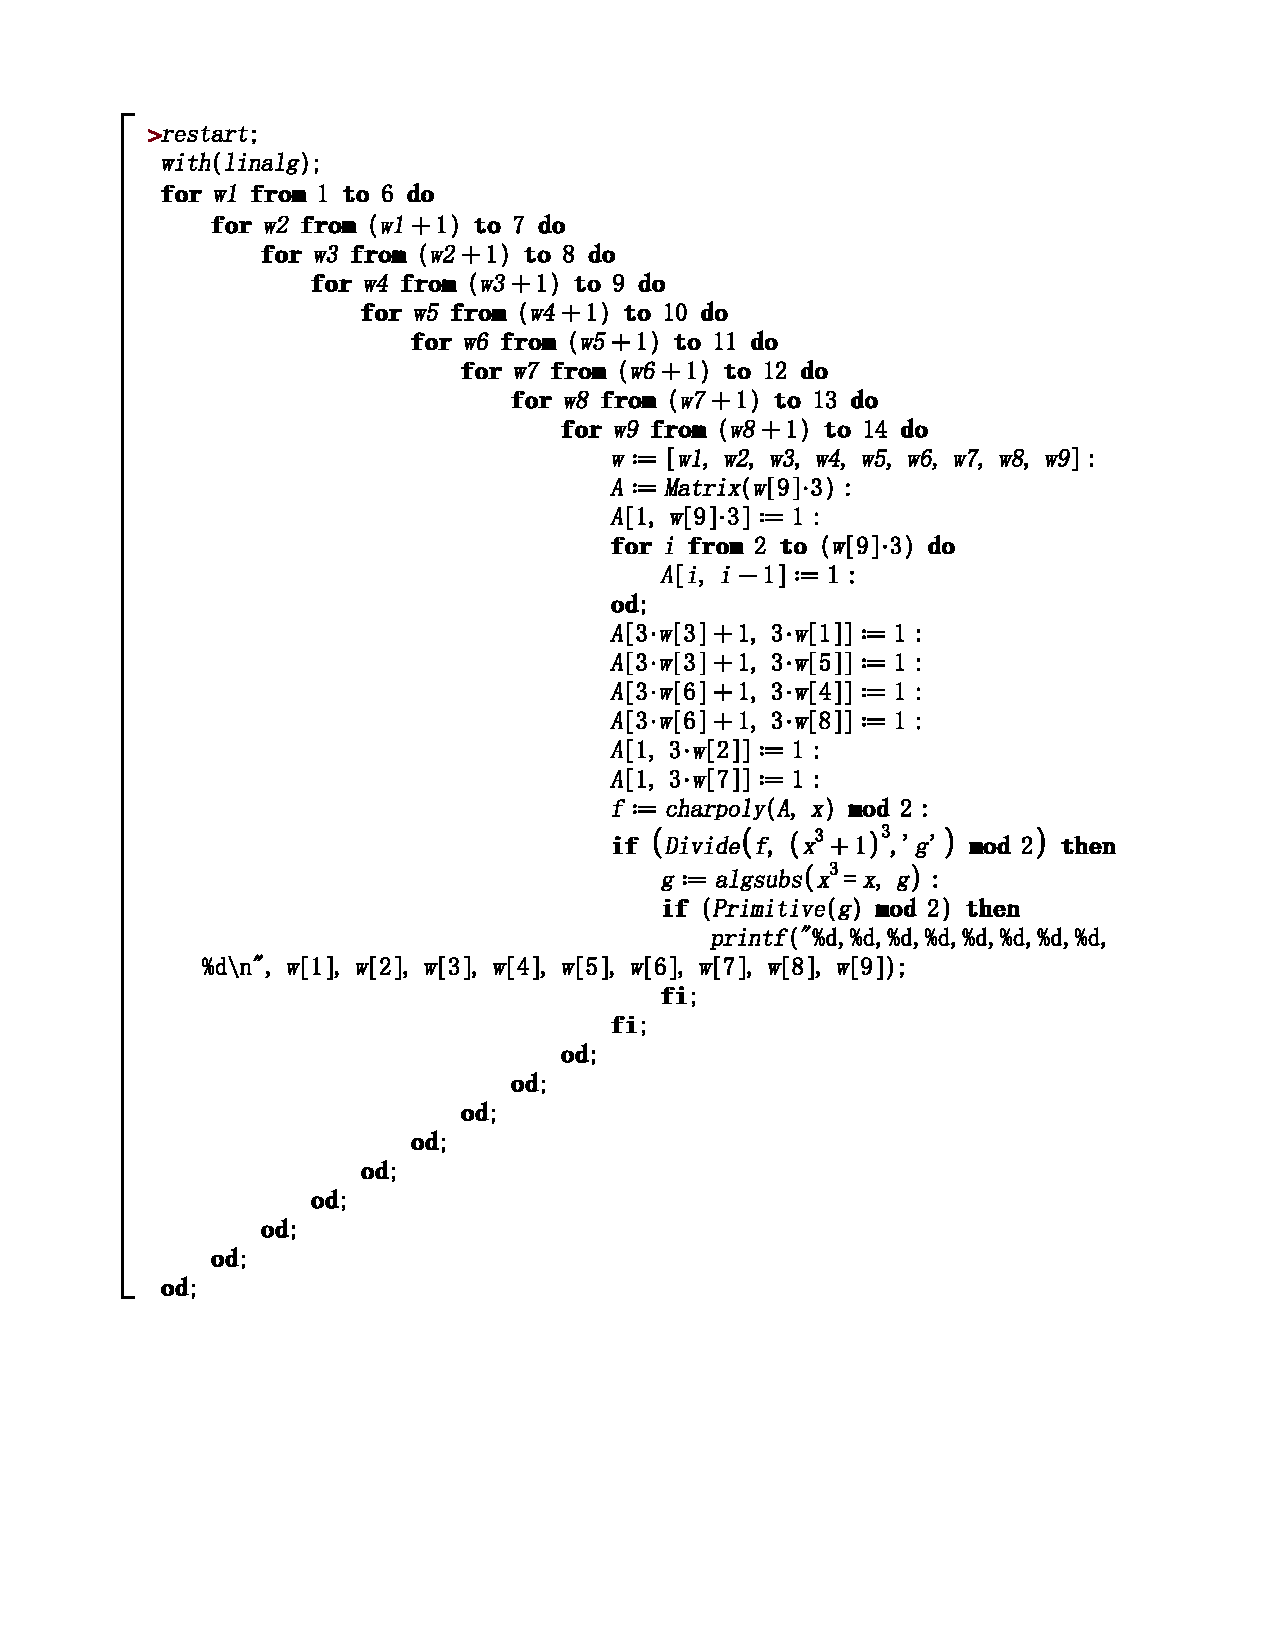
\includegraphics[width=\textwidth]{chap2/mapleTrivium.pdf}
	\caption{Trivium算法最小阶数计算}\label{fig:trivium_maple}
\end{figure}
